\section{The Coherence Pipeline: From Question to Result}
\label{sec:pipeline}

The preceding sections describe components. This section shows how they integrate
into a single coherent pipeline. The augmented democracy system is not a collection
of mechanisms but a \textit{processing pipeline} where each stage gates the next.

\subsection{The Six-Stage Pipeline}

\begin{figure}[ht]
\centering
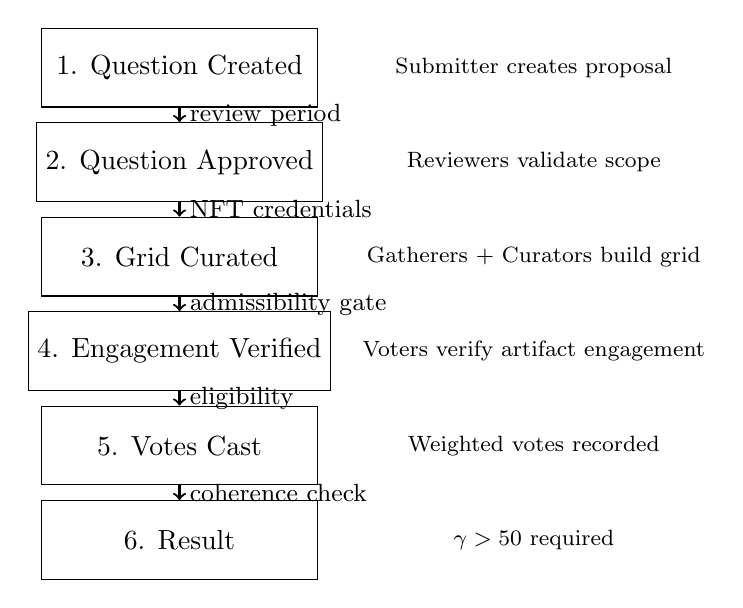
\begin{tikzpicture}[
    node distance=1.2cm,
    stage/.style={draw, rectangle, minimum width=3.5cm, minimum height=1cm, align=center},
    arrow/.style={->, thick}
]
    % Stages
    \node[stage] (q) {1. Question Created};
    \node[stage, below of=q] (a) {2. Question Approved};
    \node[stage, below of=a] (g) {3. Grid Curated};
    \node[stage, below of=g] (t) {4. Engagement Verified};
    \node[stage, below of=t] (v) {5. Votes Cast};
    \node[stage, below of=v] (r) {6. Result};

    % Arrows with labels
    \draw[arrow] (q) -- node[right, font=\small] {review period} (a);
    \draw[arrow] (a) -- node[right, font=\small] {NFT credentials} (g);
    \draw[arrow] (g) -- node[right, font=\small] {admissibility gate} (t);
    \draw[arrow] (t) -- node[right, font=\small] {eligibility} (v);
    \draw[arrow] (v) -- node[right, font=\small] {coherence check} (r);

    % Side annotations
    \node[right of=q, node distance=4.5cm, font=\footnotesize, align=left] {Submitter creates proposal};
    \node[right of=a, node distance=4.5cm, font=\footnotesize, align=left] {Reviewers validate scope};
    \node[right of=g, node distance=4.5cm, font=\footnotesize, align=left] {Gatherers + Curators build grid};
    \node[right of=t, node distance=4.5cm, font=\footnotesize, align=left] {Voters verify artifact engagement};
    \node[right of=v, node distance=4.5cm, font=\footnotesize, align=left] {Weighted votes recorded};
    \node[right of=r, node distance=4.5cm, font=\footnotesize, align=left] {$\gamma > 50$ required};

\end{tikzpicture}
\caption{The Coherence Pipeline}
\label{fig:pipeline}
\end{figure}

Each stage has a gate. Failure at any gate halts progression:

\begin{center}
\begin{tabular}{clll}
\toprule
\textbf{Stage} & \textbf{Action} & \textbf{Gate} & \textbf{On Failure} \\
\midrule
1 & Question created & Valid submitter NFT & Rejected \\
2 & Question approved & Review period passes & Held for revision \\
3 & Grid curated & Curator stake sufficient & Grid flagged \\
4 & Engagement verified & Engagement threshold met & Voter ineligible \\
5 & Vote cast & Signature valid, not duplicate & Vote rejected \\
6 & Result & $\gamma > 50$ \textbf{and} majority & No state change \\
\bottomrule
\end{tabular}
\end{center}

\subsection{Stage 1: Question Creation}

A registered \texttt{Submitter} creates a question (proposal):

\begin{lstlisting}[language=Rust]
// From lib.rs - submit_proposal
ensure!(
    matches!(participant.role, ParticipantRole::Submitter),
    Error::<T>::Unauthorized
);
\end{lstlisting}

The submitter must hold a valid credential NFT with the \texttt{Submitter} role.
Questions enter the system in \texttt{Submitted} status.

\textbf{Coherence dimension}: Credential coherence---only credentialed participants
can initiate state transitions.

\subsection{Stage 2: Question Approval}

Questions enter a mandatory review period:

\begin{lstlisting}[language=Rust]
voting_starts: current_block + T::ReviewPeriod::get(),
\end{lstlisting}

During review:
\begin{itemize}
    \item Reviewers assess question clarity and scope
    \item Duplicate or malformed questions are flagged
    \item Community can signal concerns
\end{itemize}

Questions that survive the review period advance to \texttt{ReadyForVoting}.

\textbf{Coherence dimension}: Temporal coherence---deliberation has minimum dwell time.

\subsection{Stage 3: Grid Curation}

Parallel to review, credentialed \textbf{Gatherers} and \textbf{Curators} build the test grid:

\begin{enumerate}
    \item \textbf{Gatherers} identify admissible artifacts: documents with valid provenance
    from recognized issuers (journals, agencies, standards bodies)
    \item \textbf{Curators} assemble artifacts into engagement verification grids
    \item Curators stake tokens on grid quality
    \item Grid is published and linked to the proposal
\end{enumerate}

Curators hold \texttt{Curator} credential NFTs. Their stake is slashed if grids contain
artifacts with invalid provenance, from non-recognized issuers, or that were retracted.

\textbf{Important}: Curators are \textit{not} slashed for admitting artifacts whose
conclusions are later contested or revised. The system does not adjudicate semantic
disputes---only procedural validity.

\textbf{Coherence dimension}: Procedural coherence---the artifact registry is curated
by accountable, credentialed participants with skin in the game.

\subsection{Stage 4: Engagement Verification}

Before voting, each participant must demonstrate engagement with proposal-relevant artifacts:

\begin{center}
\begin{tikzpicture}[node distance=2cm]
    \node[draw, rectangle] (voter) {Voter};
    \node[draw, rectangle, right of=voter, node distance=3cm] (grid) {Test Grid};
    \node[draw, diamond, right of=grid, node distance=3cm, aspect=2] (pass) {Pass?};
    \node[draw, rectangle, above of=pass, node distance=1.5cm] (eligible) {Eligible};
    \node[draw, rectangle, below of=pass, node distance=1.5cm] (retry) {Review \& Retry};

    \draw[->] (voter) -- (grid);
    \draw[->] (grid) -- (pass);
    \draw[->] (pass) -- node[right] {Yes} (eligible);
    \draw[->] (pass) -- node[right] {No} (retry);
    \draw[->] (retry) -| (voter);
\end{tikzpicture}
\end{center}

The engagement verification does not measure intelligence, political alignment, or
agreement with artifact conclusions. It verifies that the voter has \textit{encountered}
the admissible artifacts relevant to this proposal.

\textbf{Critical clarification}: A voter who has engaged with the evidence and
\textit{disagrees} with its conclusions still passes the gate. The system verifies
engagement, not agreement.

Passing the verification:
\begin{itemize}
    \item Updates the voter's credential NFT (engagements verified counter)
    \item Grants eligibility to vote on this specific proposal
    \item Contributes to the voter's reputation score
\end{itemize}

\textbf{Coherence dimension}: Procedural coherence---voters demonstrate engagement
with relevant artifacts before influencing outcomes.

\subsection{Stage 5: Votes Cast}

Eligible voters cast weighted votes:

\begin{lstlisting}[language=Rust]
// Weight calculation from lib.rs
let base_weight = participant.reputation;
let entropy_factor = (entropy[0] as u64 % 21) as i64 - 10;
let quantum_adjustment = (base_weight as i64 * entropy_factor) / 100;
let final_weight = (base_weight as i64 + quantum_adjustment).max(1);
\end{lstlisting}

Vote weight is a function of:
\begin{enumerate}
    \item \textbf{Reputation}: Accumulated from contributions, engagements verified, prior votes
    \item \textbf{Quadratic cost}: Multiple votes on same proposal cost $n^2$
    \item \textbf{Quantum entropy}: $\pm 10\%$ randomization prevents prediction
\end{enumerate}

Each vote consumes quantum entropy and records a quantum signature.

\textbf{Coherence dimensions}:
\begin{itemize}
    \item Influence coherence (quadratic bounds)
    \item Process coherence (entropy randomization)
\end{itemize}

\subsection{Stage 6: Result}

After the voting period, finalization computes the result:

\begin{lstlisting}[language=Rust]
// The dual condition from lib.rs
let approved = approve_weight > reject_weight
    && quantum_confidence > 50;
\end{lstlisting}

Two conditions must \textbf{both} be satisfied:

\begin{enumerate}
    \item \textbf{Democratic condition}: $w_{\text{approve}} > w_{\text{reject}}$
    \item \textbf{Coherence condition}: $\gamma > 50$
\end{enumerate}

The coherence score $\gamma$ measures entropy variance across votes:
\begin{equation}
    \gamma = \min\left(\frac{\sigma^2_\eta}{255}, 1\right) \times 100
\end{equation}

Low variance indicates correlated votes (Sybil attack, coordination).
High variance indicates independent voting (legitimate process).

\textbf{Critical clarification}: The coherence score measures \textit{process quality},
not outcome correctness. A proposal can pass with high coherence and still be ``wrong''
by external standards. The score measures whether the \textit{process} exhibited
properties consistent with legitimate deliberation, independent of proposal content.

\textbf{Coherence dimension}: Process coherence---the voting process itself
must exhibit properties of statistical independence and adequate entropy.

\subsection{The Integration Point}

The pipeline stages are not independent. Each feeds the next:

\begin{equation}
\text{Credential} \xrightarrow{\text{enables}} \text{Engagement} \xrightarrow{\text{unlocks}} \text{Vote} \xrightarrow{\text{weighted by}} \text{Reputation} \xrightarrow{\text{checked by}} \text{Coherence}
\end{equation}

Specifically:

\begin{itemize}
    \item \textbf{Engagement pass $\rightarrow$ Reputation}: Each verified engagement increments reputation
    \item \textbf{Reputation $\rightarrow$ Vote weight}: Higher reputation = higher base weight
    \item \textbf{Vote weight $\rightarrow$ Coherence}: Weight distribution affects $\gamma$
    \item \textbf{Coherence $\rightarrow$ Credential}: Failed coherence doesn't update credentials
\end{itemize}

This creates a \textit{feedback loop}: good-faith participation builds reputation,
which increases influence, which is checked by coherence, which rewards
legitimate behavior.

\subsection{Why Both Admissibility and Process Coherence}

One might ask: if voters demonstrate artifact engagement, why also check coherence?

The answer: \textbf{they protect against different attacks}.

\begin{center}
\begin{tabular}{lcc}
\toprule
\textbf{Attack} & \textbf{Blocked by Engagement} & \textbf{Blocked by $\gamma$} \\
\midrule
Unengaged voting & \checkmark & --- \\
Sybil (fake identities) & Partial & \checkmark \\
Coordinated manipulation & --- & \checkmark \\
Bribery & --- & \checkmark \\
Credential theft & --- & \checkmark \\
Bot voting & \checkmark & \checkmark \\
\bottomrule
\end{tabular}
\end{center}

\begin{itemize}
    \item \textbf{Admissibility gate} (engagement verification): Ensures voters have \textit{encountered} the relevant artifacts
    \item \textbf{Coherence gate} ($\gamma$): Ensures votes are \textit{statistically independent}
\end{itemize}

A voter who demonstrates engagement but coordinates with others will trigger low $\gamma$.
A voter who votes independently but hasn't engaged with artifacts fails the admissibility gate.
Both gates must pass for legitimate outcomes.

\subsection{The Complete Coherence Invariant}

Combining all dimensions, the system maintains a multi-dimensional coherence invariant:

\begin{definition}[Democratic Coherence]
A proposal outcome is \textbf{democratically coherent} if and only if:
\begin{enumerate}
    \item All voters held valid credentials (credential coherence)
    \item All voters demonstrated artifact engagement (procedural coherence)
    \item Vote weights were bounded by quadratic costs (influence coherence)
    \item Deliberation met minimum duration (temporal coherence)
    \item Entropy distribution showed high variance (process coherence)
    \item Majority of weighted votes approved (democratic condition)
\end{enumerate}
\end{definition}

The system rejects outcomes that satisfy some but not all conditions.
This is the ``coherence preservation'' of the central thesis:

\begin{quote}
\textbf{Democratic legitimacy is a measurable property of process quality,
independent of specific outcomes.}
\end{quote}

Majority rule is necessary but not sufficient. The coherence invariant
must also hold. The system constrains \textit{how} decisions are made,
not \textit{what} decisions must conclude.

\subsection{Pipeline Failure Modes}

Each stage can fail, with different recovery paths:

\begin{center}
\begin{tabular}{lll}
\toprule
\textbf{Stage Failure} & \textbf{Symptom} & \textbf{Recovery} \\
\midrule
1. Invalid submitter & Rejected immediately & Get credential \\
2. Review rejection & Question held & Revise and resubmit \\
3. Grid challenge & Grid invalidated & New curators assigned \\
4. Engagement failure & Voter ineligible & Engage with artifacts, retry \\
5. Vote rejection & Vote not counted & Resubmit with valid sig \\
6. $\gamma \leq 50$ & No state change & Investigate, revote \\
\bottomrule
\end{tabular}
\end{center}

Critically: \textbf{no failure corrupts state}. The system remains at $s_t$
until a coherent transition to $s_{t+1}$ is achieved.

\textbf{Important}: Coherence failure ($\gamma \leq 50$) does not indicate that
the proposal is wrong or harmful. It indicates only that the \textit{process}
exhibited statistical anomalies (coordination, manipulation, or entropy exhaustion).

\subsection{Summary: One Pipeline, Six Coherence Checks}

The augmented democracy system is a single pipeline:

\begin{center}
\fbox{Question $\rightarrow$ Approval $\rightarrow$ Grid $\rightarrow$ Engagement $\rightarrow$ Vote $\rightarrow$ Result}
\end{center}

Each transition is gated by a coherence check:

\begin{center}
\fbox{Credential $\rightarrow$ Temporal $\rightarrow$ Procedural $\rightarrow$ Procedural $\rightarrow$ Influence+Process $\rightarrow$ Process}
\end{center}

The ``underlying current'' is coherence preservation at every stage.
The system is not a voting mechanism with add-ons---it is a coherence-preserving
pipeline that happens to include voting as one stage.

This is the engineering realization of the central thesis: legitimacy
emerges from process invariants, not outcome ratification.

\textbf{The governance system constrains how decisions are made, not what decisions
must conclude.}
